\documentclass[10pt,xcolor={rgb}]{beamer}
    
    \usetheme{metropolis}
    \usepackage[utf8]{inputenc}
    
    \usepackage{appendixnumberbeamer}
    \usepackage{hyperref}
    
    \usepackage{booktabs}
    \usepackage[scale=2]{ccicons}

    
    \usepackage{pgfplots}
    \usepgfplotslibrary{dateplot}
    
    \usepackage{xspace}
    \newcommand{\themename}{\textbf{\textsc{metropolis}}\xspace}

    \usepackage{smartdiagram}
    \usesmartdiagramlibrary{additions}

    \usepackage{tikz}
    \usetikzlibrary{arrows,decorations.pathmorphing,backgrounds,fit,positioning,shapes.symbols,chains, shapes.arrows}

    \definecolor{bluei}{RGB}{83,116,191}
    \definecolor{blueii}{RGB}{207,212,232}
    \definecolor{greeni}{RGB}{135,200,81}
    \definecolor{greenii}{RGB}{216,235,207}
    \definecolor{grayi}{RGB}{160,160,160}

    \tikzset{
      myiblock/.style 2 args={
        draw=white,
        fill=#1,
        line width=1pt,
        rounded corners,
        align=center,
        text=white,
        font=\sffamily,
        text width=#2,
        minimum height=1cm
      },
      myoblock/.style={
        fill=#1,
        rounded corners,
        align=center,
        inner xsep=10pt
      },
      myserverblock/.style={
        fill=#1,
        rounded corners,
        align=center,
        inner xsep=15pt,
        inner ysep=6pt,
        draw=white,
      },
      myminiblock/.style 2 args={
        draw=white,
        fill=#1,
        line width=1pt,
        rounded corners,
        align=center,
        text=white,
        font=\sffamily,
        text width=#2,
        minimum height=0.5cm,
      },
    }

    \usepackage{graphicx}
    \graphicspath{ {img/} }


    \title{Control de versions}
    \subtitle{Introducció als sistemes de gestió de canvis}
    \date{27/06/2018}
    \author{Josep Maria Pinyol Fontseca}
    \institute{Endepro Software, S.L.}
    % \titlegraphic{\hfill\includegraphics[height=1.5cm]{logo.pdf}}

    \begin{document}

    \maketitle
    
    \begin{frame}{Continguts}
      \setbeamertemplate{section in toc}[sections numbered]
      \tableofcontents[hideallsubsections]
    \end{frame}
    
    
    \section{Introducció}    
    
    \begin{frame}[fragile]{Presentació}

      \begin{block}{Qui sóc?}

        %Em dic \textbf{Josep Maria Pinyol Fontseca} i sóc un apassionat de la programació. Aquí a la UPC em van ensenyar a programar microprocesadors, però la curiositat d’entendre què hi havia darrera d’aquella programació, ara fa més de 20 anys, em va encaminar al desenvolupament de software. Des de fa 14 anys dirigeixo els projectes que desenvolupa el meu equip a Endepro Software
        Em dic \textbf{Josep Maria Pinyol Fontseca} i sóc un apassionat de la programació. De formació Enginyer Industrial en Electrònica, vaig començar a programar microprocesadors, però la curiositat d’entendre què hi havia darrera d’aquella programació, ara fa més de 20 anys, em va encaminar al desenvolupament de software. Des de fa 14 anys dirigeixo els projectes que desenvolupa el meu equip a Endepro Software

        \centering
        
\includegraphics[width=2cm, height=2cm]{endepro.png}
      \end{block}

    \end{frame}


    \begin{frame}[fragile]{Introducció}

      \begin{block}{Qué és un sistema de control de versions?}
        \begin{itemize}
          \item Gestió de canvis d'arxius en el temps
          \item Revertir un arxiu a una versió anterior de forma simple
          \item Comparar canvis en el temps
          \item Visualitzar qui ha realitzat determinats canvis en un fitxer
          \item S'utilitza principalment a la industria informàtica
        \end{itemize}
      \end{block}
      
    \end{frame}

    \section{Sistemes de control de versions}
    
    \begin{frame}[fragile]{Sistema de control habitural}

      Un dels primers sistemes de control de versions els coneixem perfectament. 
      \begin{block}{Segurament molts de nosaltres hem fet això més d'una vegada:}
      \begin{itemize}
        \item Oferta.docx
        \item Oferta-Copia.docx
        \item Oferta-Copia (2).docx
        \item Oferta-BO.docx
        \item Oferta-BO-2.docx
      \end{itemize}
      \end{block}
      I quina és l'oferta bona?
    \end{frame}

    \begin{frame}[fragile]{Sistema de control habitural}
      
      \begin{block}{Si sóm molt organitzats inclourem la data i hora en el nom del fitxer:}
            
            \begin{itemize}
              \item Oferta-18-6-2017-17:20.docx
              \item Oferta-18-6-2017-17:25.docx
              \item Oferta-19-6-2017-8:42.docx
              \item Oferta-19-6-2017-9:15.docx
            \end{itemize}

      \end{block}
      El mateix pasa amb projectes sencers que estan en una carpeta, fent versions de les carpetes, etc.
    \end{frame}
          
    \begin{frame}[fragile]{Per què necessitem un sistema de control de versions?}
      
      \begin{block}{Però, per què realment necessitem un sistema de control de versions:}
            
            \begin{itemize}
              \item Còpia i restauració:  podem saltar a una versió del dia que vulguem
              \item Sincronització: podem compartir els fitxers i tenir la última versió
              \item Desfer a curt termini:  podem tirar enrera dels canvis que hem anat fent durant els últims dies
              \item Desfer a llarg termini:  si necessitem una versió de fa 1 any, cap problema
              \item Control de canvis:  controlar tots els canvis que es fan en els fitxers 
              \item Control dels usuaris:  tenim el nom i cognoms de qui ha fet el canvi
              \item Branques i unions:  si volem fer molts canvis en un projecte, podem aïllar el nostre codi, fer els canvis i unir-ho tot un cop estigui fet
            \end{itemize}

      \end{block}

    \end{frame}

    \begin{frame}[fragile]{Tipus de Sistemes de control de versions}
      
            
      \begin{block}{Evolució i generacions dels sistemes de control de versions:}
        
        \begin{enumerate}
          \item Sistemes de control de versions locals
          \item Sistemes de control de versions centralitzats
          \item Sistemes de control de versions distribuïts
        \end{enumerate}

      \end{block}

    \end{frame}
      
    \begin{frame}[fragile]{Sistemes de control de versions locals}
      
      \begin{block}{Primera generació: local}
        
        \begin{itemize}
          \item Disponible per a sistemes UNIX des del 1972
          \item Disenyat per controlar els canvis realitats en el codi font o fitxers de text
          \item Tenim disponible el RCS per vàries plataformes
        \end{itemize}

      \end{block}

      \begin{center}
        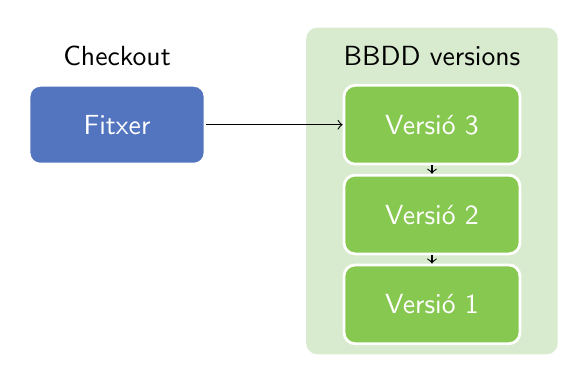
\begin{tikzpicture}[node distance=0.5cm and 1cm]
          \node[myiblock={bluei}{2cm}]
            (info1)
            {Fitxer};
          \node[above=3pt of info1,font=\sffamily]
            (title1)
            {Checkout};

          \begin{scope}[xshift=4cm,node distance=3pt and 1cm]
          \node[myiblock={greeni}{2cm}]
            (infoob1)
            {Versió 3};
          \node[myiblock={greeni}{2cm},below=of infoob1]
            (infoob2)
            {Versió 2};
          \node[myiblock={greeni}{2cm},below=of infoob2]
            (infoob3)
            {Versió 1};
          \node[above=3 pt of infoob1,font=\sffamily]
            (title2)
            {BBDD versions};
          \begin{pgfonlayer}{background}
          \node[myoblock=greenii,fit={(title2) (infoob3)}] {};  
          \end{pgfonlayer}
          \end{scope}

          \draw [->] (info1) edge (infoob1);
          \draw [->] (infoob1) edge (infoob2) (infoob2) edge (infoob3);
        \end{tikzpicture}
      \end{center}

    \end{frame}

    \begin{frame}[fragile]{Sistemes de control de versions centralitzat}

      \begin{block}{Segona generació: centralitzat}
        
        \begin{itemize}
          \item Disponible des del 1986
          \item Arquitectura client servidor
          \item Les implementacions més utilitzades són: CVS, Subversion (SVN)
        \end{itemize}

      \end{block}

      \begin{center}
        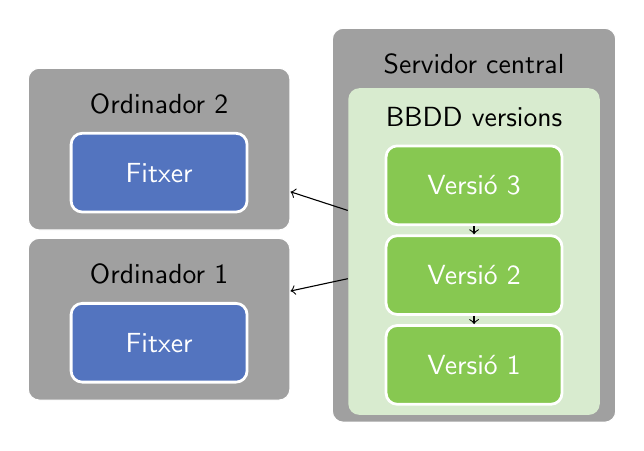
\begin{tikzpicture}[node distance=0.5cm and 1cm]

          \node[myiblock={bluei}{2cm}]
            (fitxer1)
            {Fitxer};
          \node[above=3pt of fitxer1,font=\sffamily]
            (ordinador1)
            {Ordinador 1};

          \node[above=15pt of ordinador1, myiblock={bluei}{2cm}]
            (fitxer2)
            {Fitxer};
          \node[above=3pt of fitxer2,font=\sffamily]
            (ordinador2)
            {Ordinador 2};

          \begin{pgfonlayer}{background}
            \node[myserverblock=grayi,fit={(fitxer2) (ordinador2)}] (repoord1) {};  
          \end{pgfonlayer}

          \begin{pgfonlayer}{background}
            \node[myserverblock=grayi,fit={(fitxer1) (ordinador1)}] (repoord2) {};  
          \end{pgfonlayer}

          \begin{scope}[yshift=2cm, xshift=4cm,node distance=3pt and 1cm]
          \node[myiblock={greeni}{2cm}]
            (infoob1)
            {Versió 3};
          \node[myiblock={greeni}{2cm},below=of infoob1]
            (infoob2)
            {Versió 2};
          \node[myiblock={greeni}{2cm},below=of infoob2]
            (infoob3)
            {Versió 1};
          \node[above=3 pt of infoob1,font=\sffamily]
            (title2)
            {BBDD versions};
          \node[above=5 pt of title2,font=\sffamily]
            (title3)
            {Servidor central};         
            
            \begin{pgfonlayer}{background}
              \node[myserverblock=grayi,fit={(title3) (infoob3)}] {};  
            \end{pgfonlayer}
            
          \begin{pgfonlayer}{background}
          \node[myoblock=greenii,fit={(title2) (infoob3)}] (repo) {};  
          \end{pgfonlayer}

          \end{scope}

          \draw [->] (repo) edge (repoord1);
          \draw [->] (repo) edge (repoord2);
          \draw [->] (infoob1) edge (infoob2) (infoob2) edge (infoob3);
        \end{tikzpicture}
      \end{center}
    
    
    \end{frame}

    \begin{frame}[fragile]{Sistemes de control distribuït}

      \begin{block}{Tercera generació: distribuït}
        
        \begin{itemize}
          \item Disponible des del 2000
          \item Arquitectura desentralitzada o distribuïda
          \item Les implementacions més utilitzades són: GIT, Mercurial (HG)
        \end{itemize}

        \begin{center}
          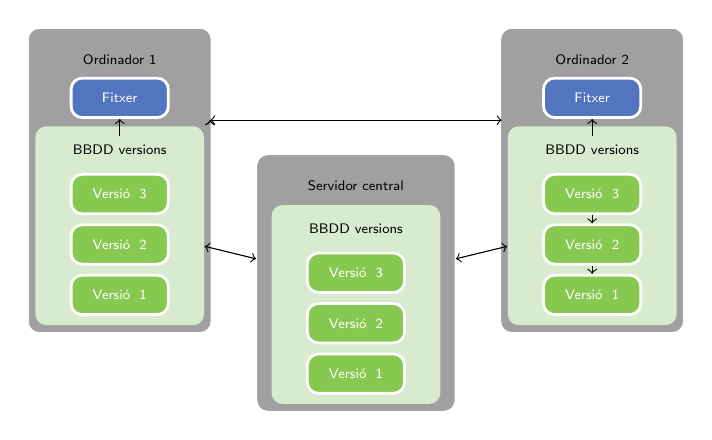
\begin{tikzpicture}[node distance=0.5cm and 1cm]

            %Servidor central
            \begin{scope}[xshift=4cm,node distance=3pt and 1cm]
            \node[myminiblock={greeni}{1cm}]
              (infoob1)
              {\tiny Versió 3};
            \node[myminiblock={greeni}{1cm},below=of infoob1]
              (infoob2)
              {\tiny Versió 2};
            \node[myminiblock={greeni}{1cm},below=of infoob2]
              (infoob3)
              {\tiny Versió 1};
            \node[above=3 pt of infoob1,font=\sffamily]
              (title2)
              {\tiny BBDD versions};

              \node[above=5 pt of title2,font=\sffamily]
              (title3)
              {\tiny Servidor central};         
              
              \begin{pgfonlayer}{background}
                \node[myserverblock=grayi,fit={(title3) (infoob3)}] (backServer) {};  
              \end{pgfonlayer}

              \begin{pgfonlayer}{background}
              \node[myoblock=greenii,fit={(title2) (infoob3)}] {};  
              \end{pgfonlayer}

            \end{scope}

            %Ordinador 1
            \begin{scope}[yshift=1cm,xshift=1cm,node distance=3pt and 1cm]
              \node[myminiblock={greeni}{1cm}]
                (infoob1)
                {\tiny Versió 3};
              \node[myminiblock={greeni}{1cm},below=of infoob1]
                (infoob2)
                {\tiny Versió 2};
              \node[myminiblock={greeni}{1cm},below=of infoob2]
                (infoob3)
                {\tiny Versió 1};
              \node[above=3 pt of infoob1,font=\sffamily]
                (title2Ordinador1)
                {\tiny BBDD versions};
  
                \node[myminiblock={bluei}{1cm}, above=6pt of title2Ordinador1]
                (fitxerOrdinador1)
                {\tiny Fitxer};    
  
                \node[above=1 pt of fitxerOrdinador1,font=\sffamily]
                (title3)
                {\tiny Ordinador 1};         
   
                
                \begin{pgfonlayer}{background}
                  \node[myserverblock=grayi,fit={(title3) (infoob3)}] {};  
                \end{pgfonlayer}
  
                \begin{pgfonlayer}{background}
                \node[myoblock=greenii,fit={(title2Ordinador1) (infoob3)}] (backOrdinador1) {};  
                \end{pgfonlayer}
  
            \end{scope}

            %Ordinador 2
            \begin{scope}[yshift=1cm,xshift=7cm,node distance=3pt and 1cm]
              \node[myminiblock={greeni}{1cm}]
                (infoob1)
                {\tiny Versió 3};
              \node[myminiblock={greeni}{1cm},below=of infoob1]
                (infoob2)
                {\tiny Versió 2};
              \node[myminiblock={greeni}{1cm},below=of infoob2]
                (infoob3)
                {\tiny Versió 1};
              \node[above=3 pt of infoob1,font=\sffamily]
                (title2Ordinador2)
                {\tiny BBDD versions};

                \node[myminiblock={bluei}{1cm}, above=6pt of title2Ordinador2]
                (fitxerOrdinador2)
                {\tiny Fitxer};    
  
                \node[above=1 pt of fitxerOrdinador2,font=\sffamily]
                (title3)
                {\tiny Ordinador 2};         
                
                \begin{pgfonlayer}{background}
                  \node[myserverblock=grayi,fit={(title3) (infoob3)}] {};  
                \end{pgfonlayer}
  
                \begin{pgfonlayer}{background}
                \node[myoblock=greenii,fit={(title2Ordinador2) (infoob3)}] (backOrdinador2) {};  
                \end{pgfonlayer}
  
            \end{scope}
  
            \draw [->] (infoob1) edge (infoob2) (infoob2) edge (infoob3);
            \draw [->] (title2Ordinador2) edge (fitxerOrdinador2);
            \draw [->] (title2Ordinador1) edge (fitxerOrdinador1);
            \draw [<->] ([yshift=2pt, xshift=2pt] backOrdinador1.north east) edge ([yshift=2pt, xshift=-2pt] backOrdinador2.north west);
            \draw [<->] (backOrdinador1) edge (backServer);
            \draw [<->] (backOrdinador2) edge (backServer);
            
          \end{tikzpicture}
        \end{center}

      \end{block}

    \end{frame}



    \begin{frame}[fragile]{Argot}
      
            \begin{block}{Argot general}
      
              \begin{itemize}
                \item Repositori (repo): base de dades amb els fitxers  
                \item Servidor: ordinador on hi ha el repositori
                \item Client:  ordinador que es connecta al repositori
                \item Trunk/Main/Master: primera localització del codi en el repositori
              \end{itemize}
            \end{block}
      
    \end{frame}

    \begin{frame}[fragile]{Argot}
      
            \begin{block}{Accions en sistemes centralitzats}
      
              \begin{itemize}
                \item Checkout:  descarregar fitxers o fitxer del repositori
                \item Add:  afegir un fitxer/fitxers en el repositori per primer cop
                \item Check in: carregar fitxers al repositori
                \item ChangeLog/History:  llista de canvis fets a un fitxer
                \item Update/Sync: sincronitza els fitxers locals a la última versió del repositori
                \item Revert: descarta els canvis locals del fitxer i agafa la última versió del repositori
              \end{itemize}
            \end{block}
      
    \end{frame}

    \begin{frame}[fragile]{Argot}
      
            \begin{block}{Accions en sistemes distribuïts}
      
              \begin{itemize}
                \item Pull:  obtenir canvis d'un altre repositori
                \item Push:  enviar canvis a un altre repositori
                \item Commit: enviar canvis al repositori local 
             \end{itemize}
            \end{block}
      
    \end{frame}

    \begin{frame}[fragile]{Argot}
      
            \begin{block}{Accions avançades}
      
              \begin{itemize}
                \item Branch: crea una copia separada per per test, correccions, etc.
                \item Diff: diferencia entre dos fitxers
                \item Merge (Path): aplica canvis d'un fitxer a un altre per tenir la última versió
                \item Conflict: al tenir canvis pendents que contradiuen un altre canvi (els dos canvis no es poden aplicar)
                \item Resolve:  resolució dels conflictes
              \end{itemize}
            \end{block}
      
    \end{frame}


    \begin{frame}[fragile]{Revisions}
      
            \begin{block}{Revisions}
      
              \begin{itemize}
                \item Cada cop que fem una nova versió tenim una nova revisió del fitxer
              \end{itemize}

              \centering
              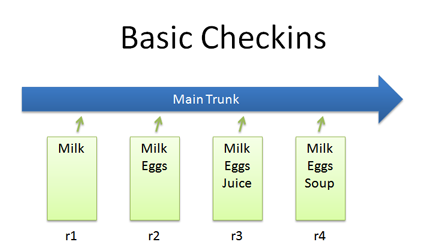
\includegraphics[height=4cm]{basic_checkin.png}
      
            \end{block}
      
    \end{frame}

    \begin{frame}[fragile]{Revisions en sistemes centralitzats}
      
            \begin{block}{Revisions en un sistema centralitzat}
      
              \begin{itemize}
                \item Els diferents desenvolupadors envien els canvis a la branca principal
                \item Teòricament s'hauria de fer una branca perque els altres ho provin
              \end{itemize}

              \centering
              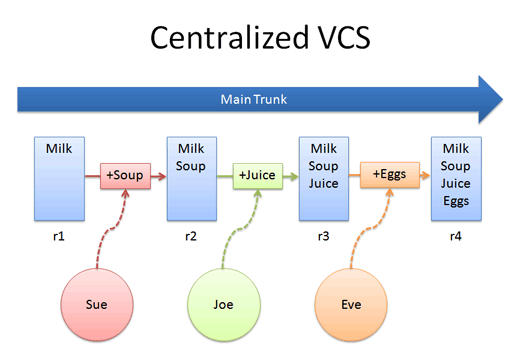
\includegraphics[height=4cm]{centralized_example.png}
      
            \end{block}
      
    \end{frame}

    \begin{frame}[fragile]{Canvis i edició}
      
            \begin{block}{Canvis i edició}
      
              \begin{itemize}
                \item En realitat obtenir la revisió, editem i guardem la revisió
                \item Podem desfer els canvis a una revisió anterior sempre que vulguem
              \end{itemize}

              \centering
              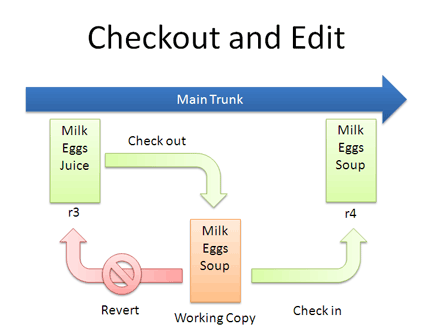
\includegraphics[height=4cm]{checkout_edit.png}
      
            \end{block}
      
    \end{frame}

    \begin{frame}[fragile]{Diferències}
      
            \begin{block}{Diferències}
      
              \begin{itemize}
                \item Es guarden les diferències entres revisions
                \item La majoria de sistemes de control de versions guarden aquests diferencies en comptes de tots els fitxers
              \end{itemize}

              \centering
              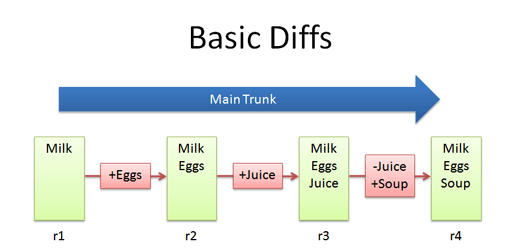
\includegraphics[height=4cm]{basic_diffs.png}
      
            \end{block}
      
    \end{frame}


    \begin{frame}[fragile]{Branques}
      
            \begin{block}{Branques}
      
              \begin{itemize}
                \item Les branques ens permeten fer una còpia del codi en una "carpeta" diferent
                
              \end{itemize}

              \centering
              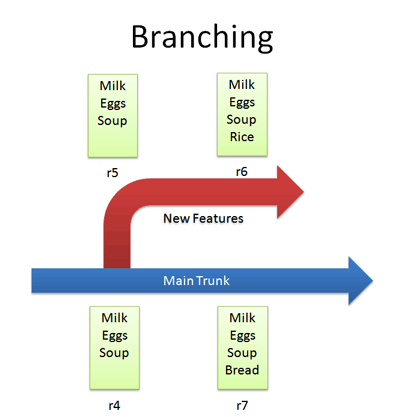
\includegraphics[height=6cm]{first_branch.png}
      
            \end{block}
      
    \end{frame}


    \begin{frame}[fragile]{Unions o Merge}
      
            \begin{block}{Merge}
      
              \begin{itemize}
                \item En permet unir canvis realitzats de branques diferents
                
              \end{itemize}

              \centering
              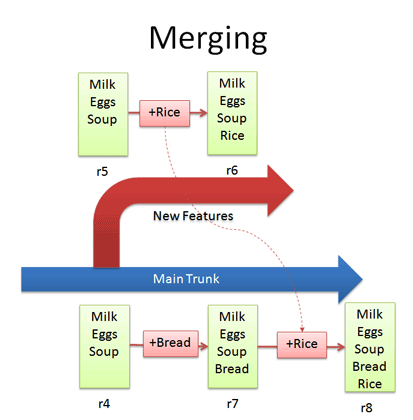
\includegraphics[height=6cm]{merging.png}
      
            \end{block}
      
    \end{frame}

    \begin{frame}[fragile]{Conflictes}
      
            \begin{block}{Conflictes}
      
              \begin{itemize}
                \item A vegades les unions o merges ens donen conflictes en el codi
                
              \end{itemize}

              \centering
              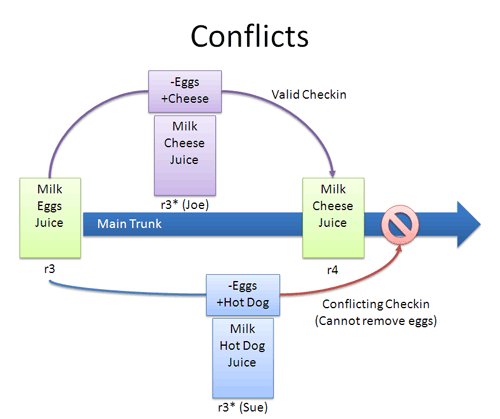
\includegraphics[height=6cm]{vcs_conflict.png}
      
            \end{block}
      
    \end{frame}
    
    \begin{frame}[fragile]{Etiquetes o Tags}
      
            \begin{block}{Etiquetes o Tags}
      
              \begin{itemize}
                \item Podem marcar la revisió per tenir una etiqueta identificativa de la revisió
                
              \end{itemize}

              \centering
              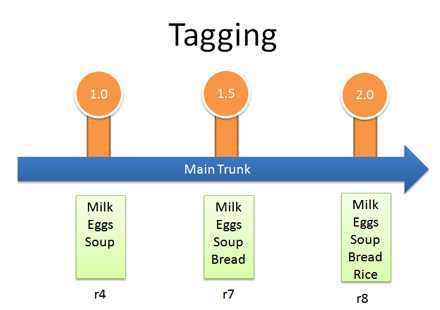
\includegraphics[height=6cm]{tagging.png}
      
            \end{block}
      
    \end{frame}

    \begin{frame}[fragile]{Introducció als sistemes distribuïts}
      
            \begin{block}{En sistemes distribuïts cada desenvolupador té el seu propi repo}
      
              \begin{itemize}
                \item En sistemes distribuïts es fan unions entre les branques dels desenvolupadors
                
              \end{itemize}

              \centering
              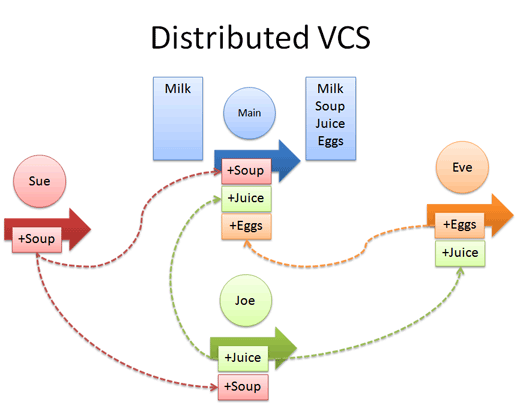
\includegraphics[height=6cm]{distributed_example.png}
      
            \end{block}
      
    \end{frame}  

    \begin{frame}[fragile]{Merge en sistemes distribuïts}
      
            \begin{block}{Merge en sistemes distribuïts}
      
              \begin{itemize}
                \item En sistemes distribuïts es fan unions entre les branques dels desenvolupadors
                
              \end{itemize}

              \centering
              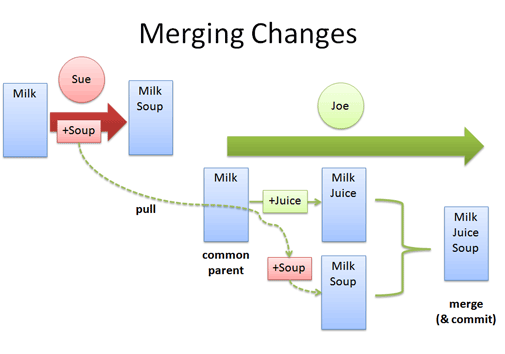
\includegraphics[height=6cm]{distributed_merge.png}
      
            \end{block}
      
    \end{frame}  

    \begin{frame}[fragile]{Organització d'un projecte en sistemes distribuïts}
      
            \begin{block}{Organització d'un projecte en sistemes distribuïts}
      
              \begin{itemize}
                \item Els programadors comproven els canvis en una branca comuna
                \item El responsable revisa els canvis i ho envia a la branca stable
              \end{itemize}

              \centering
              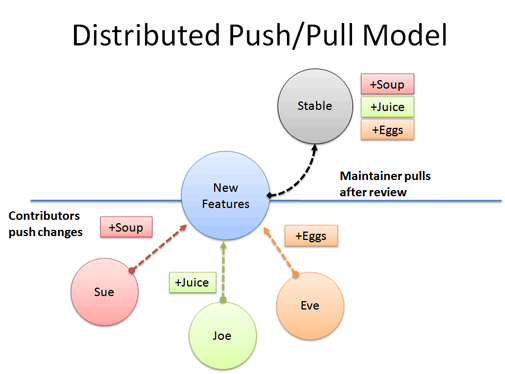
\includegraphics[height=6cm]{distributed_push_pull.png}
      
            \end{block}
      
    \end{frame}  

    \begin{frame}[fragile]{Avantatges del sistema Distribuït vs Centralitzat}
      
            \begin{block}{Principals avantatges del sistema distribuït:}
      
              \begin{itemize}
                \item Tothom té una còpia local del codi
                \item Es pot treballar Offline
                \item És ràpid, tot es fa localment i no en el servidor central
                \item Els canvis es gestionen millor al tenir un GUID per canvi realitzat
                \item Les Branques i les Unions són fàcils ja que cada desenvolupador té la seva pròpia Branca i es poden realitzar proves fàcilment
                \item Menys gestió, ja que no cal un servidor central en funcionament
              \end{itemize}
      
            \end{block}
      
    \end{frame}

    \section{Pràctiques}
    
    \begin{frame}[fragile]{GIT - Sistema de control de versions distribuït}
            \begin{block}{Utilitzarem GIT com a sistema de control de versions}
      
              \begin{itemize}
                \item La majoria d'entorns de desenvolupament i editors ja tenen integrat el GIT
                \item Es pot treballar amb linia de comandes o amb programes especifics per GIT
                \item Per començar, descarregar i instal·lar https://git-scm.com/downloads
              \end{itemize}
      
            \end{block}
    \end{frame}

    \begin{frame}[fragile]{GIT}
      \begin{block}{Inicialització d'un repositori}

        \begin{enumerate}
          \item \texttt{\textbf{git init}}
          \item Si ens hi fixem ens ha creat una carpeta \textbf{.git} en el directori de treball
          \item Ja tenim el repositori apunt

        \end{enumerate}

      \end{block}
    \end{frame}

    \begin{frame}[fragile]{GIT}
      \begin{block}{Inicialització d'un repositori - Configuració}

        \begin{enumerate}
          \item Anem a configurar les dades de l'usuari que treballa amb el control de versions
          \item Nom: \texttt{\textbf{git config --global user.nom "Josep Maria Pinyol Fontseca" }}
          \item Correu: \texttt{\textbf{git config --global user.email "jmpinyol@endepro.com" }}

        \end{enumerate}

      \end{block}
    \end{frame}

    \begin{frame}[fragile]{GIT}
      \begin{block}{Afegim fitxers al repositori creat i ho enviem al repositori}

        \begin{enumerate}
          \item \texttt{\textbf{git add fitxer.txt}}
          \item \texttt{\textbf{git commit -m "Versió inicial del fitxer"}}
        \end{enumerate}

      \end{block}
    \end{frame}

    \begin{frame}[fragile]{GIT}
      \begin{block}{Fluxe de treball general}

        \centering
        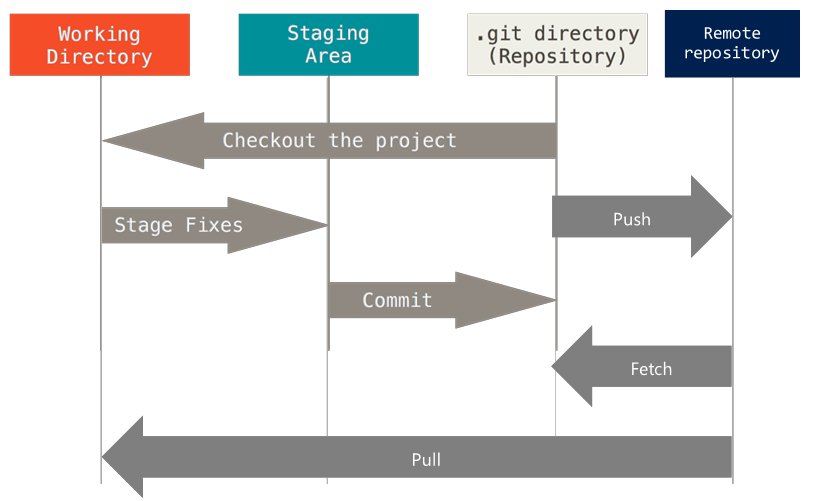
\includegraphics[height=6cm]{git.png}

      \end{block}
    \end{frame}

    \begin{frame}[fragile]{GIT}
      \begin{block}{Modificant i enviant els fitxers modificats}

        \begin{enumerate}
          \item Modifiquem el contingut del fitxer.txt
          \item \texttt{\textbf{git status}} ens dona informació de l'estat actual
          \item \texttt{\textbf{git add fitxer.txt}}
          \item \texttt{\textbf{git commit -m "Canvis que he fet..."}}
        \end{enumerate}

      \end{block}
    \end{frame}

    \begin{frame}[fragile]{GIT}
      \begin{block}{Modificant i recuperar la versió anterior}

        \begin{enumerate}
          \item Modifiquem el contingut del fitxer.txt de nou
          \item \texttt{\textbf{git checkout fitxer.txt}}
          \item Tornem a tenir la versió anterior del fitxer
          \item Podem revertir un commit sencer amb un revert \texttt{\textbf{git revert master}}
        \end{enumerate}

      \end{block}
    \end{frame}

    \begin{frame}[fragile]{GIT}
      \begin{block}{Visualització d'estat}

        \begin{enumerate}
          \item Tenim diferents instruccions per tenir informació del repositori, directori de treball, etc.
          \item Per saber l'estat del directori actual: \texttt{\textbf{git status}} 
          \item Si volem un registre dels commits realitzats \texttt{\textbf{git log}}
          \item Amb \texttt{\textbf{git blame fitxer}} ens dona informació d'un fitxer en concret
        \end{enumerate}

      \end{block}
    \end{frame}

    \begin{frame}[fragile]{GIT}
      \begin{block}{Modificant, stage i unstage d'un fitxer en concret}

        \begin{enumerate}
          \item Modifiquem el contingut del fitxer.txt de nou
          \item \texttt{\textbf{git commit fitxer.txt}}
          \item \texttt{\textbf{git status}}
          \item \texttt{\textbf{git reset HEAD fitxer.txt}}
          \item El fitxer l'hem afegit per enviar al repositori però al final l'hem tret
        \end{enumerate}

      \end{block}
    \end{frame}

    \begin{frame}[fragile]{GIT}
      \begin{block}{Treballant amb etiquetes}

        \begin{enumerate}
          \item \texttt{\textbf{git tag -a 1.0 -m "Versió 1.0"}}
          \item \texttt{\textbf{git tag}}
        \end{enumerate}

        

      \end{block}
    \end{frame}

    \begin{frame}[fragile]{GIT}
      \begin{block}{Treballant amb branques}

        \begin{enumerate}
          \item \texttt{\textbf{git branch testing}}
        \end{enumerate}

        \centering
        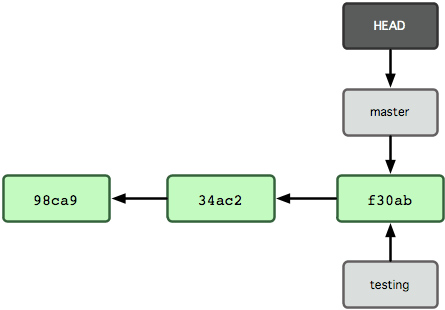
\includegraphics[height=6cm]{b1.png}

      \end{block}
    \end{frame}

    \begin{frame}[fragile]{GIT}
      \begin{block}{Treballant amb branques}

        \begin{enumerate}
          \item \texttt{\textbf{git checkout testing}}
        \end{enumerate}

        \centering
        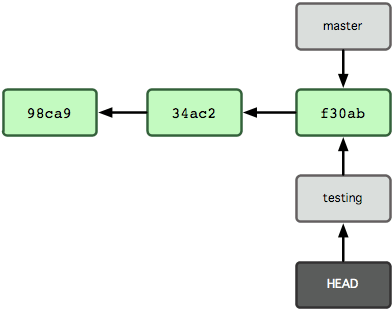
\includegraphics[height=6cm]{b2.png}

      \end{block}
    \end{frame}

    \begin{frame}[fragile]{GIT}
      \begin{block}{Treballant amb branques}

        \begin{enumerate}
          \item Modifiquem el fitxer.txt i ho enviem al repositori
        \end{enumerate}

        \centering
        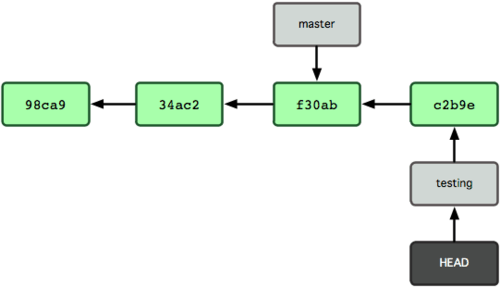
\includegraphics[height=6cm]{b3.png}

      \end{block}
    \end{frame}

    \begin{frame}[fragile]{GIT}
      \begin{block}{Treballant amb branques}

        \begin{enumerate}
          \item Tornem a la branca master
          \item \texttt{\textbf{git checkout master}}
        \end{enumerate}

        \centering
        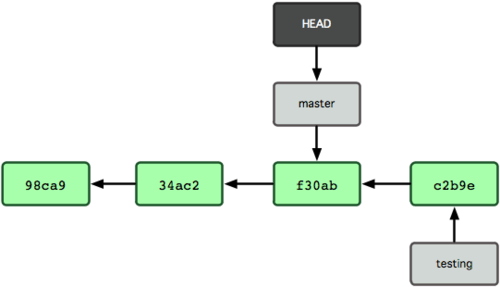
\includegraphics[height=6cm]{b4.png}

      \end{block}
    \end{frame}

    \begin{frame}[fragile]{GIT}
      \begin{block}{Treballant amb branques}

        \begin{enumerate}
          \item Modifiquem el fitxer.txt i ho enviem al repositori
        \end{enumerate}

        \centering
        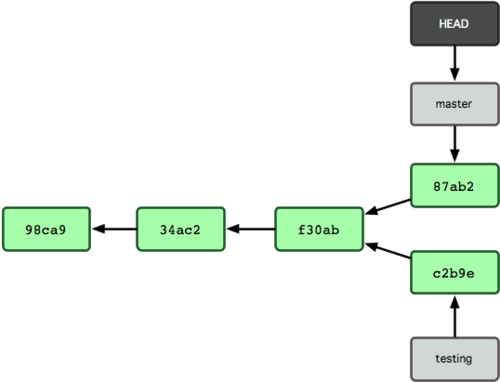
\includegraphics[height=6cm]{b5.png}

      \end{block}
    \end{frame}

    \begin{frame}[fragile]{GIT}
      \begin{block}{Treballant amb branques - Merge}

        \begin{enumerate}
          \item Entrem a la branca testing i afegim un nou fitxer
          \item Si canviem de branca veurem que en una hi ha uns fitxers diferents que en l'altra
          \item \texttt{\textbf{git checkout master}}
          \item \texttt{\textbf{git merge testing}}
        \end{enumerate}

      \end{block}
    \end{frame}

    \begin{frame}[fragile]{GIT}
      \begin{block}{Treballant amb branques - Conflictes}

        \begin{enumerate}
          \item Entrem a la branca testing, modifiquem el fitxer.txt en una mateixa linia que la master i l'enviem al repo
          \item \texttt{\textbf{git checkout testing}}
          \item \texttt{\textbf{git add fitxer.txt}}
          \item \texttt{\textbf{git commit -m "Desde de testing"}}
          \item Saltem a la branca master i fem un merge
          \item \texttt{\textbf{git checkout master}}
          \item \texttt{\textbf{git merge testing}}
        \end{enumerate}

      \end{block}
    \end{frame}

    \begin{frame}[fragile]{GIT}
      \begin{block}{Treballant amb branques}

        \begin{enumerate}
          \item Anem a recuperar una versió anterior (d'un TAG)
          \item \texttt{\textbf{git checkout 1.0 -b branca1.0}}
          \item Fem els canvis pertinents
          \item \texttt{\textbf{git commit -m "Desde de 1.0"}}
          \item Saltem a la branca master i fem un merge
          \item \texttt{\textbf{git checkout master}}
          \item \texttt{\textbf{git merge branca1.0}}
        \end{enumerate}

      \end{block}
    \end{frame}


    \begin{frame}[fragile]{GIT}
      \begin{block}{Treballant amb branques - Detached HEAD}

        \begin{enumerate}
          \item Podem anar a un commit en concret.  En aquest cas, el HEAD no apuntarà a cap branca
          \item \texttt{\textbf{git checkout 1.0}}
          \item Estem en Detached HEAD state.  Els commits, etc no es guardaran
          \item Per tornar a l'estat normal fem un \texttt{\textbf{git checkout master}}
          \item És millor fer una branca i treballar en aquesta.  Sempre la podem esborrar un cop provat el que vulguem
        \end{enumerate}

      \end{block}
    \end{frame}

    \begin{frame}[fragile]{GIT}
      \begin{block}{Treballant amb branques - Esborrar branques}

        \begin{enumerate}
          \item Moltes vegades podem fer branques per provar o corregir problemes en el projecte
          \item Un cop fet i tenim el merge realitzat, podem esborrar-la amb un \texttt{\textbf{git branch -d testing}}
        \end{enumerate}

      \end{block}
    \end{frame}

    \begin{frame}[fragile]{GIT}
      \begin{block}{Excloure fitxers}

        \begin{enumerate}
          \item Podem excloure fitxers utilitzant el fitxer \texttt{\textbf{.gitignore}}
          \item Com a exemple, creem el fitxer test.exe
          \item l'afegim al \texttt{\textbf{.gitignore}}
          \item Si fem un \texttt{\textbf{git status}} no apareix
          \item Afegit el \texttt{\textbf{.gitignore}} al repostitori
          \item A la URL https://github.com/github/gitignore tenim fitxers ignore comuns per tipus de projectes
        \end{enumerate}

      \end{block}
    \end{frame}

    \begin{frame}[fragile]{GIT}
      \begin{block}{Pràctica}

        \begin{enumerate}
          \item Crear el projecte "Test" de tipus consola els Visual Studio 2017 (C\#) i afegir-ho a un repositori GIT
        \end{enumerate}

      \end{block}
    \end{frame}

    \begin{frame}[fragile]{GIT}
      \begin{block}{Stash}

        \begin{enumerate}
          \item Podem acumular els canvis que hem fet per utilitzar més endavant
          \item Fem alguns canvis el fitxer
          \item Executem \texttt{\textbf{git stash}} i tornarem a tenir el fitxer anterior
          \item Podem tenir més d'un stash a la cua.  Podem veure la llista amb \texttt{\textbf{git stash list}}
          \item Per \texttt{\textbf{git stash list}}
          \item Per agafar un stash \texttt{\textbf{git stash pop}} o \texttt{\textbf{git stash pop stash@{2}}}
          \item Tenir en compte que fa un merge amb l'actual
        \end{enumerate}

      \end{block}
    \end{frame}


    \begin{frame}[fragile]{GIT}
      \begin{block}{Connexió amb repositoris remots}

        \begin{enumerate}
          \item Anem a descarregar un repositori remot
          \item \texttt{\textbf{git clone http...}}
          \item Ja tenim una copia del repositori remot en local
          \item A partir d'aqui podem treballar localment sense necessitat de connexió
        \end{enumerate}

      \end{block}
    \end{frame}

    \begin{frame}[fragile]{GIT}
      \begin{block}{Enviar canvis al respositori central}

        \begin{enumerate}
          \item Afegim algun fitxer al repositori
          \item Fem un Commit
          \item Enviem els canvis al respositori central: \texttt{\textbf{git push}}
        \end{enumerate}

      \end{block}
    \end{frame}

    \begin{frame}[fragile]{GIT}
      \begin{block}{Rebre canvis}

        \begin{enumerate}
          \item Abans de rebre canvis hem de fer un \textbf{commit} del nostre repositori local  
          \item Fem un Pull per rebre els canvis: \texttt{\textbf{git pull}}
          \item Si volem rebre tota la informació del repositori podem fer un fetch \texttt{\textbf{git fetch}}
        \end{enumerate}

      \end{block}
    \end{frame}




    \section{Utilitzant un gestor GIT}
    
    \begin{frame}[fragile]{Gestor GIT}
      \begin{block}{Treballar amb un gestor GIT}

        No és fàcil treballar per linia de comandes i alguns editors o entorns tenen un gestor GIT limitat
        \begin{itemize}
          \item Utilitzar un gestor GIT que ens ajudi en el dia a dia
          \item Tenim moltes opcions:  SmartGit, GitKraken, SourceTree, TortoiseGIT, etc.
        \end{itemize}

      \end{block}
    \end{frame}

        
    \begin{frame}[fragile]{Gestor GIT}
      \begin{block}{Treballar amb un gestor GIT}

        Treballarem amb el SourceTree ja que utilitzem BitBucket i queda tot més integrat.
        \begin{itemize}
          \item Descarregar la última versió de https://www.sourcetreeapp.com
        \end{itemize}

      \end{block}
    \end{frame}

    \begin{frame}[fragile]{Gestor GIT - Pràctica}
      \begin{block}{Pràctica}

        \begin{enumerate}
          \item Crearem un projecte on hi participi varis usuaris
          \item Primer un usuari serà el crearà l'estructura bàsica del projecte i el publicarà en un repositori
          \item La resta d'usuaris farà una part del projecte
        \end{enumerate}

      \end{block}
    \end{frame}
    
    \begin{frame}[standout]
      Preguntes?
    \end{frame}

    \begin{frame}{}
      Gràcies per la vostra assistència
    \end{frame}
    
\end{document}
    